% Compile with pdfLaTeX (twice). All diagrams are editable TikZ source.
\documentclass[12pt,a4paper]{article}
\usepackage[T1]{fontenc}
\usepackage[utf8]{inputenc}
\usepackage{lmodern}
\usepackage[margin=1in]{geometry}
\usepackage{amsmath,amssymb,graphicx}
\usepackage{tikz}
\usetikzlibrary{arrows.meta,positioning,calc,fit,backgrounds,shapes.geometric}
\usepackage{array,enumitem}
\usepackage{caption,float}
\usepackage[hidelinks]{hyperref}
\hypersetup{pdftitle={ICMP Smurf Attack: Design and Security Analysis},pdfauthor={Dip Saha; MD. Mehedi Hasan Mim}}
\newcommand{\CourseName}{Security Sessional (CSE 406)}
\newcommand{\InstructorName}{Anwarul Bashir Shuaib}
\newcommand{\DepartmentName}{Department of Computer Science and Engineering}
\newcommand{\UniversityName}{Bangladesh University of Engineering and Technology}
\newcommand{\SubmissionDate}{September 12, 2026}
\renewcommand{\thesection}{\arabic{section}}
\renewcommand{\thesubsection}{\thesection.\arabic{subsection}}
\setlength{\parindent}{0pt}
\setlength{\parskip}{6pt}
\setlist{leftmargin=*,itemsep=4pt,topsep=4pt}
\renewcommand{\arraystretch}{1.25}
\definecolor{TableHeader}{HTML}{12304A}
\definecolor{TableShade}{HTML}{F5F7F9}
\definecolor{TableRule}{HTML}{C9D2DA}
\newcolumntype{Y}{>{\raggedright\arraybackslash}X}
\newcolumntype{L}[1]{>{\raggedright\arraybackslash}m{#1}}
\newcommand{\tablehead}[1]{\textcolor{white}{\bfseries #1}}
\captionsetup{font=small,labelfont=bf,skip=6pt}
\setlength{\intextsep}{10pt}
\tikzset{box/.style={draw=black,rounded corners=2pt,fill=white,align=center,minimum height=0.8cm,font=\small},req/.style={-{Latex[length=2.5mm]},thick},rep/.style={-{Latex[length=2.5mm]},thick},life/.style={densely dashed,gray},lab/.style={font=\footnotesize,align=center,fill=white,inner sep=3pt}}
\begin{document}
\begin{titlepage}
\centering
\vspace*{1.2in}
{\Large\bfseries Bangladesh University of Engineering and Technology\par}
\vspace{0.25in}
{\large\bfseries Department of Computer Science and Engineering\par}
\vspace{0.9in}
{\Large\bfseries CSE 406 --- Security Sessional\par}
\vspace{0.55in}
{\LARGE\bfseries ICMP Smurf Attack\par}
\vspace{0.2in}
{\Large Design Report\par}
\vspace{0.8in}
\begin{tabular}{ll}
\textbf{Submitted by:} & \\
Dip Saha & Student ID: 2105138\\
MD. Mehedi Hasan Mim & Student ID: 2105142\\[0.4in]
\textbf{Supervised by:} & \\
Anwarul Bashir Shuaib & Lecturer, Department of CSE, BUET
\end{tabular}
\vfill
{\large September 12, 2026\par}
\end{titlepage}
\pagenumbering{roman}
\tableofcontents
\clearpage
\pagenumbering{arabic}

\section{Overview of the Project Idea}
An \textbf{ICMP Smurf attack} is a reflection-and-amplification Denial-of-Service (DoS) attack that abuses the interaction between IP source-address spoofing, directed-broadcast delivery, and hosts that respond to ICMP Echo Requests. Instead of sending a large volume of packets directly to the victim, the attacker sends requests to an amplifier network while forging the victim's IP address as the source.

The key idea is simple. A single spoofed ICMP Echo Request can be delivered to many hosts when it targets a directed broadcast address. If $N$ hosts respond, the victim receives up to $N$ Echo Replies for one attacker-generated request. Repeating this process creates a many-to-one traffic pattern that can consume the victim's bandwidth, packet-processing capacity, or both.

The project studies the attack as a protocol-level security problem rather than as a software vulnerability. The ICMP packet itself can be completely well-formed; the abuse comes from the meaning of its addressing and the network behavior around it. The report therefore focuses on the protocol fields involved, the packet flow, the assumptions that make the attack possible, and defenses that remove those assumptions.

\textbf{Project objective.} Demonstrate the classic Smurf mechanism only inside an isolated, controlled laboratory network, then identify the observable indicators and configure defenses that prevent spoofed requests, directed-broadcast reflection, or broadcast ICMP responses.

\textbf{Core security properties under study}
\begin{itemize}
\item \textbf{Source authenticity:} IPv4 source addresses are not inherently authenticated.
\item \textbf{Broadcast fan-out:} a directed broadcast can deliver one IP datagram to multiple hosts when the network permits it.
\item \textbf{Reflection:} ICMP Echo Replies are addressed to the apparent source of the request.
\item \textbf{Amplification:} multiple responders transform one request into multiple replies.
\item \textbf{Availability impact:} the resulting traffic is directed toward the victim and can interfere with legitimate service.
\end{itemize}

\section{Background: ICMP Echo, IP Broadcast, and Smurfing}
The Internet Control Message Protocol (ICMP) is used by IP hosts and routers for control, diagnostic, and error-reporting functions. ICMP Echo Request and Echo Reply are commonly exposed through the \texttt{ping} utility. In IPv4, an Echo Request uses \textbf{Type 8, Code 0}; a successful Echo Reply uses \textbf{Type 0, Code 0}. The Echo Reply normally copies the request's identifier, sequence number, and data so that the sender can associate the reply with the original request.

The Smurf attack relies on a special destination rather than a normal unicast destination. For a subnet such as \texttt{203.0.113.0/24}, the directed broadcast address is \texttt{203.0.113.255}. A router configured to forward directed broadcasts can deliver a packet addressed to that network-wide destination to the hosts on the destination LAN.

The second ingredient is source-address spoofing. The attacker places the victim's IP address in the source field of the Echo Request. The amplifier hosts therefore see the victim as the apparent sender. If they answer the request, their Echo Replies are sent to the victim.

Historically, this combination produced the classic Smurf attack. Modern networks commonly disable directed-broadcast forwarding and suppress responses to broadcast or multicast Echo Requests. Network operators also use source-address validation to reduce the ability of attackers to transmit packets with forged source addresses.

\subsection{Why the attack is possible}
The attack does not require a malformed ICMP message. Instead, it exploits three independent configuration assumptions:
\begin{enumerate}
\item the attacker's network allows a packet with a forged source address to leave;
\item the amplifier network forwards the directed broadcast; and
\item enough hosts respond to the broadcast Echo Request.
\end{enumerate}
Removing any one of these assumptions significantly weakens or breaks the classic reflection path.

\subsection{Amplification model}
Let $R$ be the attacker's rate of spoofed Echo Requests and $N$ the number of amplifier hosts that respond to each request. In an idealized lossless model, the victim receives approximately
\[
R_{\mathrm{victim}} \approx N R
\]
Echo Replies per second. The packet-count amplification factor is therefore
\[
A_{\mathrm{packets}}=\frac{NR}{R}=N.
\]
This is an ideal upper-bound model: packet loss, host rate limits, filtering, and incomplete participation reduce the observed amplification.

\section{Threat Model and Assumptions}
The attacker is assumed to control a host that can generate IPv4/ICMP traffic but does not have administrative access to the victim or the amplifier hosts. The attacker does not need to compromise the amplifier machines. They are unwitting participants whose network configuration causes them to respond.

The victim is an IP host or service whose network capacity or protocol stack is targeted by the reflected Echo Replies. The amplifier network is a third-party subnet containing multiple responsive hosts. The attacker may be geographically and topologically separate from that network.

\begin{center}
\small
\begin{tabular}{@{}p{3.6cm} p{11.8cm}@{}}
\hline
\textbf{Role} & \textbf{Assumption}\\
\hline
Attacker & Can transmit IP packets and, in the vulnerable scenario, can spoof the source address of the victim.\\
Amplifier network & Has a directed-broadcast address and permits the broadcast to reach multiple hosts.\\
Amplifier hosts & Respond to broadcast ICMP Echo Requests rather than silently discarding them.\\
Victim & Receives the reflected Echo Replies and has finite bandwidth, processing, and buffering resources.\\
Network & Provides an IP forwarding path from the attacker to the amplifier network and from the amplifiers to the victim.\\
\hline
\end{tabular}
\end{center}

\subsection{Scope and safety assumptions}
The project implementation is intended for an isolated virtual laboratory. Example addresses in this report use documentation-only IPv4 ranges and are not intended to identify real systems. No public network, third-party host, or production infrastructure should be used for the demonstration.

The attacker's objective in the model is \textbf{availability disruption}. Confidentiality, credential theft, malware installation, and modification of application data are outside the scope of this project.

\section{Network Topology and Components}
The laboratory scenario models three logical components: an attacker, an amplifier/bounce network, and a victim. The amplifier network contains several hosts that are configured to respond to broadcast Echo Requests. The example addressing below is illustrative and uses documentation address space.

\begin{figure}[H]
\centering
% ===== topology =====
% Figure 1: Smurf topology. All example addresses are illustrative.
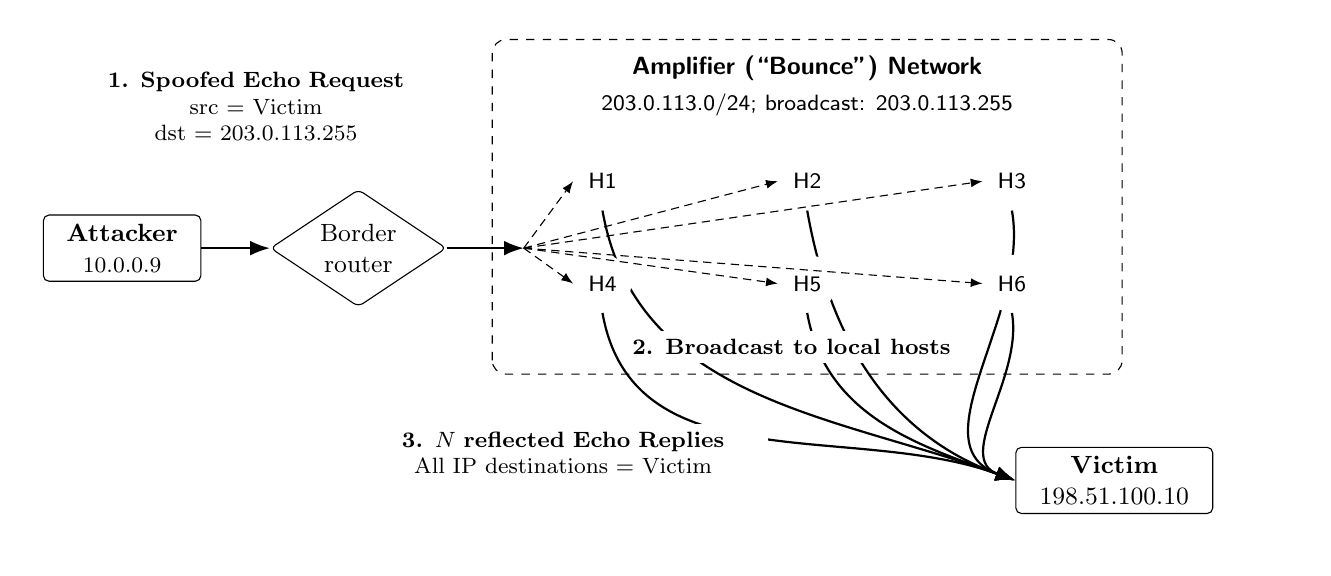
\begin{tikzpicture}[x=1cm,y=1cm]
\path[use as bounding box] (-.1,-.5) rectangle (16.1,6.1);
\filldraw[fill=white,dashed,rounded corners=5pt] (5.8,1.7) rectangle (13.8,5.95);
\node[font=\sffamily\small\bfseries] at (9.8,5.58) {Amplifier (``Bounce'') Network};
\node[font=\sffamily\footnotesize] at (9.8,5.12) {203.0.113.0/24; broadcast: 203.0.113.255};
\node[box,minimum width=2cm] (a) at (1.1,3.3) {\textbf{Attacker}\\\footnotesize 10.0.0.9};
\node[box,diamond,aspect=1.5,inner sep=2pt] (r) at (4.1,3.3) {Border\\router};
\node[box,minimum width=2.5cm] (v) at (13.7,.35) {\textbf{Victim}\\198.51.100.10};
\draw[req] (a)--(r);
\coordinate (b) at (6.2,3.3);
\draw[req] (r)--(b);
\foreach \name/\xx/\yy in {H1/7.2/4.15,H2/9.8/4.15,H3/12.4/4.15,H4/7.2/2.85,H5/9.8/2.85,H6/12.4/2.85}{
\node[circle,fill=white,minimum size=.7cm,font=\sffamily\footnotesize] (\name) at (\xx,\yy) {\name};
\draw[densely dashed,-{Latex[length=1.5mm]}] (b)--(\name.west);
\draw[rep] (\name.south) to[out=-80,in=160] (v.west);
}
\node[lab,text width=5.2cm] at (2.8,5.1) {\textbf{1. Spoofed Echo Request}\\src = Victim\\dst = 203.0.113.255};
\node[lab] at (9.6,2.05) {\textbf{2. Broadcast to local hosts}};
\node[lab,text width=5cm] at (6.7,.7) {\textbf{3. $N$ reflected Echo Replies}\\All IP destinations = Victim};
\end{tikzpicture}

\caption{Topology of the Smurf attack. Blue arrows show request delivery; red arrows show reflected replies. The victim sees replies originating from the amplifier hosts.}
\end{figure}

\textbf{Actors and components}

\begin{center}
\begin{tabular}{@{}p{3.6cm} p{11.8cm}@{}}
\hline
\textbf{Component} & \textbf{Purpose} \\
\hline
Attacker & Generates the controlled ICMP Echo Request traffic with the victim's address as the apparent source. \\
Border router & Represents the routing point that may permit or deny directed-broadcast forwarding. \\
Amplifier network & Receives the directed broadcast and distributes it to the local broadcast domain. \\
Amplifier hosts $H_1,\ldots,H_N$ & Respond to the Echo Request and generate reflected Echo Replies. \\
Victim & Receives the aggregate replies and is the endpoint whose availability is evaluated. \\
\hline
\end{tabular}
\end{center}

The important property of the topology is that the attacker does not need to send a separate packet to each amplifier. The broadcast mechanism performs the fan-out. Conversely, the amplifier hosts do not need to know the attacker's identity; they simply respond to the source address carried in the request.

\section{Attack Methodology}
The attack can be understood as four phases. The first phase establishes the packet's source and destination conditions; the second causes network-wide delivery inside the amplifier subnet; the third produces reflected replies; and the fourth repeats the process to create sustained traffic.

\subsection{Phase 1 --- Source-address spoofing}
The attacker creates an ICMP Echo Request whose source IP address is the victim's IP address. The ICMP Type and Code remain normal values (8 and 0). The important manipulation occurs in the IPv4 source field. If source-address filtering is absent, the packet can be forwarded even though the source does not represent the actual sender.

\subsection{Phase 2 --- Directed-broadcast delivery}
The destination is the directed broadcast address of the amplifier network. For a \texttt{/24} network, this is the address with the final eight host bits set to one. A router that permits directed-broadcast forwarding delivers the request to the local broadcast domain, where multiple hosts can receive the same IP datagram.

\subsection{Phase 3 --- Reflection}
Each amplifier host that accepts the broadcast request constructs an ICMP Echo Reply addressed to the apparent source address. Because the request's source is the victim, the replies converge on the victim rather than returning to the attacker.

\subsection{Phase 4 --- Repetition and amplification}
The attacker repeats the spoofed requests at a controlled rate. If $N$ hosts respond to each request, the victim can receive approximately $N$ replies per request in the ideal model. Multiple amplifier networks can further increase the aggregate number of responders, although real networks introduce filtering, loss, and rate limiting.

\textbf{Attack chain:}\quad
\textit{spoof victim source}
$\rightarrow$
\textit{target directed broadcast}
$\rightarrow$
\textit{many hosts respond}
$\rightarrow$
\textit{replies converge on victim}
$\rightarrow$
\textit{repeat for sustained load}.

\subsection{Why the design works}
\textbf{Spoofed source.} IPv4 does not cryptographically authenticate the source-address field. Without effective source validation, the amplifier hosts cannot infer the true sender from the source field alone.

\textbf{Broadcast destination.} The directed broadcast turns one packet into multiple host deliveries. The attacker does not need to enumerate every amplifier host individually.

\textbf{Reflected flood.} Each responding host independently generates an Echo Reply. At a fixed request rate, more responders mean more packets arriving at the victim. Larger ICMP payloads increase bytes per packet, while the number of responders primarily determines the packet-count amplification.

\section{Timing Diagrams}
\subsection{The protocol as it normally behaves}
Under normal operation, ICMP Echo is a one-to-one request/response exchange. Host A sends an Echo Request to Host B, and Host B sends one Echo Reply back to A.

\begin{figure}[H]
\centering
% ===== normal-timing =====
% Figure 2: Normal unicast exchange; time increases downwards.
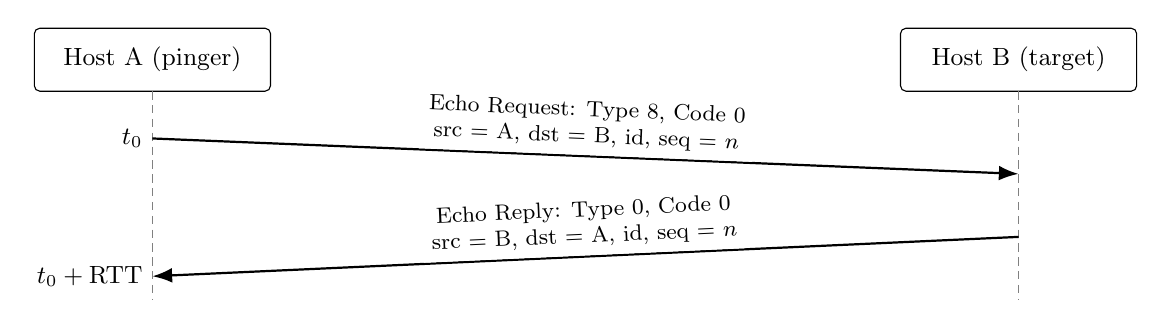
\begin{tikzpicture}[x=1cm,y=1cm]
\node[box,minimum width=3cm] at (2,0) {Host A (pinger)};
\node[box,minimum width=3cm] at (13,0) {Host B (target)};
\draw[life] (2,-.4)--(2,-3.05);
\draw[life] (13,-.4)--(13,-3.05);
\node[left,font=\small] at (2,-1) {$t_0$};
\node[left,font=\small] at (2,-2.75) {$t_0+\mathrm{RTT}$};
\draw[req] (2,-1)--node[lab,above,sloped]{Echo Request: Type 8, Code 0\\src = A, dst = B, id, seq = $n$}(13,-1.45);
\draw[rep] (13,-2.25)--node[lab,above,sloped]{Echo Reply: Type 0, Code 0\\src = B, dst = A, id, seq = $n$}(2,-2.75);
\end{tikzpicture}

\caption{Benign ICMP echo timing: a single round trip between the true source and destination. RTT denotes round-trip time.}
\end{figure}

\subsection{The Smurf attack}
During the attack, the one-to-one exchange is replaced by a one-to-many request followed by many-to-one responses. The request is addressed to the amplifier network's broadcast address and uses the victim as its apparent source.

\begin{figure}[H]
\centering
% ===== attack-timing =====
% Figure 3: Repeated reflection; the fan of three arrows symbolizes N replies.
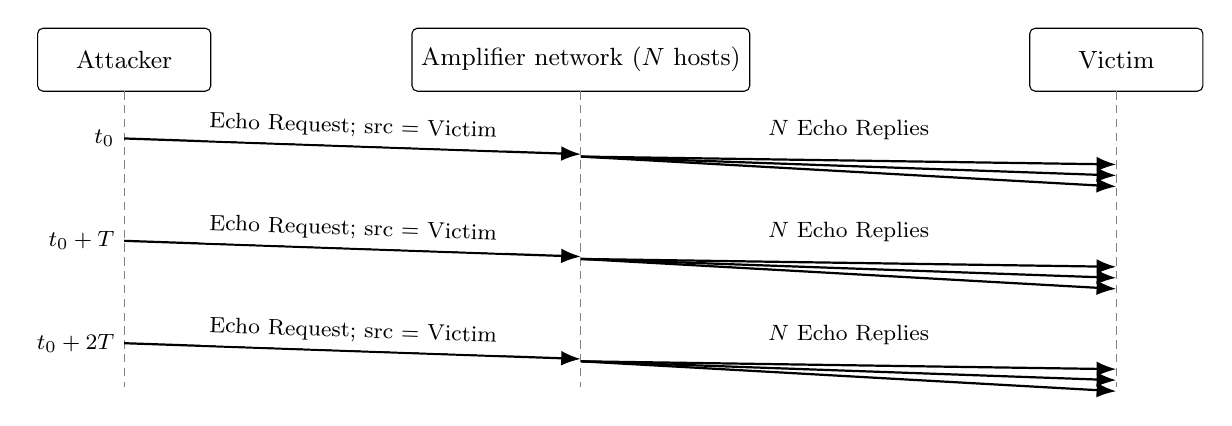
\begin{tikzpicture}[x=1cm,y=1cm]
\node[box,minimum width=2.2cm] at (1.2,0) {Attacker};
\node[box,minimum width=4cm] at (7,0) {Amplifier network ($N$ hosts)};
\node[box,minimum width=2.2cm] at (13.8,0) {Victim};
\foreach \x in {1.2,7,13.8}{\draw[life] (\x,-.4)--(\x,-4.15);}
\foreach \y/\t in {-1/t_0,-2.3/{t_0+T},-3.6/{t_0+2T}}{
\node[left,font=\footnotesize] at (1.2,\y) {$\t$};
\draw[req] (1.2,\y)--node[lab,above,sloped]{Echo Request; src = Victim}(7,\y-.2);
\foreach \d in {0,.14,.28}{\draw[rep] (7,\y-.23) -- (13.8,\y-.33-\d);}
\node[lab,above] at (10.4,\y-.13) {$N$ Echo Replies};
}
\end{tikzpicture}

\caption{Attack timing. Each request triggers up to $N$ replies. Repetition every $T$ seconds sustains amplified traffic; arrival times depend on network delay and host response time.}
\end{figure}

The timing is not necessarily perfectly simultaneous: each amplifier host may process the request at a slightly different time, and the replies can experience different queuing and propagation delays. Nevertheless, the aggregate traffic pattern is a burst or stream of unsolicited Echo Replies converging on the victim.

\section{Packet and Frame Structure}
The attack packet is an ordinary IPv4 datagram carrying an ICMP Echo Request. No malformed packet format is necessary. The security-relevant changes are the IPv4 source and destination addresses; ICMP Type and Code remain those of a normal Echo Request.

\subsection{IPv4 Header}
\begin{figure}[H]
\centering
% ===== ipv4-header =====
% Figure 4: Accurate 32-bit-wide IPv4 header grid (no options).
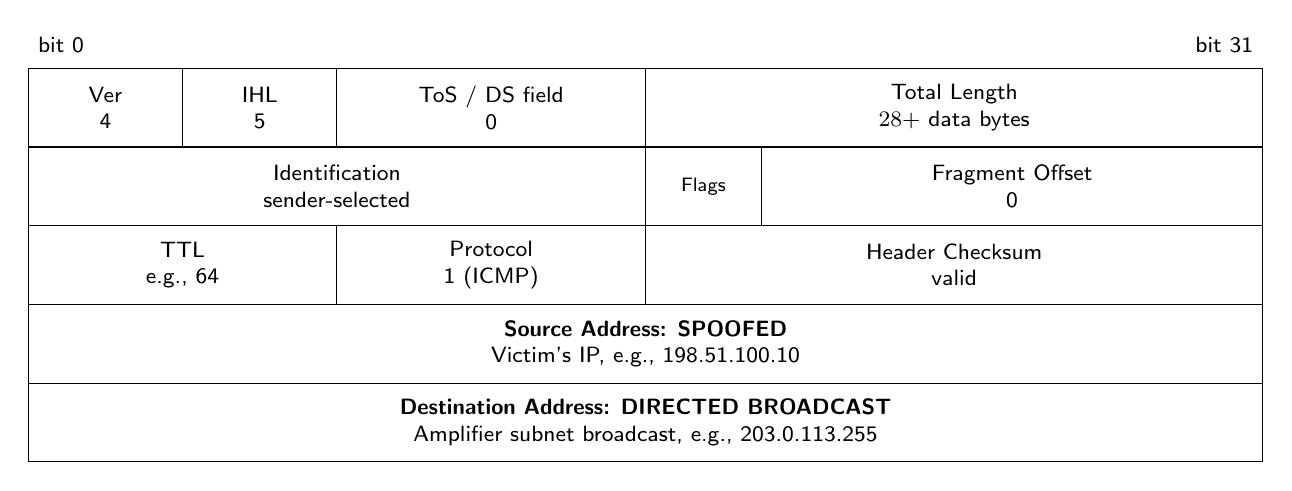
\begin{tikzpicture}[x=.49cm,y=1cm,font=\sffamily\footnotesize]
\node[anchor=west] at (0,.3) {bit 0};
\node[anchor=east] at (32,.3) {bit 31};
\fill[white] (0,0) rectangle (32,-3);
\fill[white] (0,-3) rectangle (32,-5);
\draw (0,0) rectangle (32,-5);
\foreach \y in {-1,-2,-3,-4}{\draw (0,\y)--(32,\y);}
\foreach \x in {4,8,16}{\draw (\x,0)--(\x,-1);}
\foreach \x in {16,19}{\draw (\x,-1)--(\x,-2);}
\foreach \x in {8,16}{\draw (\x,-2)--(\x,-3);}
\node[align=center] at (2,-.5) {Ver\\4};
\node[align=center] at (6,-.5) {IHL\\5};
\node[align=center] at (12,-.5) {ToS / DS field\\0};
\node[align=center] at (24,-.5) {Total Length\\$28+$ data bytes};
\node[align=center] at (8,-1.5) {Identification\\sender-selected};
\node[align=center,font=\sffamily\scriptsize] at (17.5,-1.5) {Flags};
\node[align=center] at (25.5,-1.5) {Fragment Offset\\0};
\node[align=center] at (4,-2.5) {TTL\\e.g., 64};
\node[align=center] at (12,-2.5) {Protocol\\1 (ICMP)};
\node[align=center] at (24,-2.5) {Header Checksum\\valid};
\node[align=center] at (16,-3.5) {\textbf{Source Address: SPOOFED}\\Victim's IP, e.g., 198.51.100.10};
\node[align=center] at (16,-4.5) {\textbf{Destination Address: DIRECTED BROADCAST}\\Amplifier subnet broadcast, e.g., 203.0.113.255};
\end{tikzpicture}

\caption{IPv4 header of the outbound attack packet, assuming a 20-byte header without options. The two address fields implement spoofing and directed broadcast delivery.}
\end{figure}

\subsection{ICMP Header and Payload}
\begin{figure}[H]
\centering
% ===== icmp-header =====
% Figure 5: ICMP Echo header; variable-length data is shown schematically.
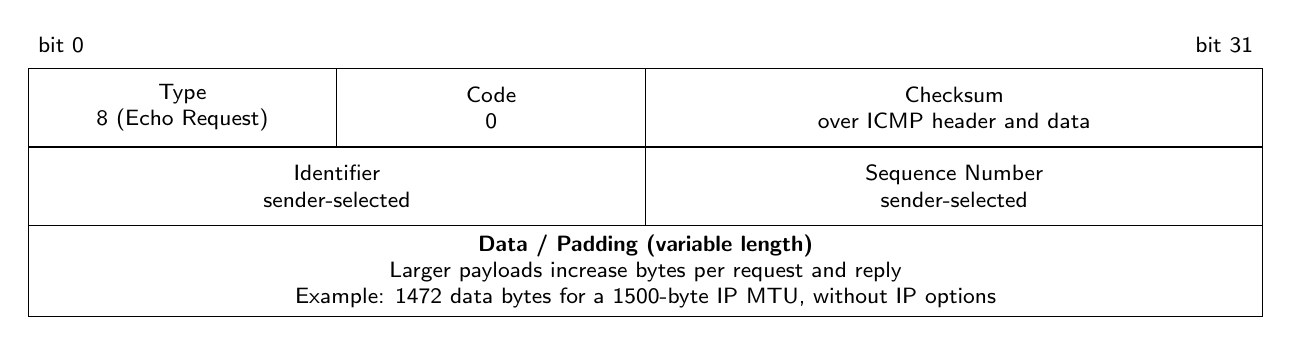
\begin{tikzpicture}[x=.49cm,y=1cm,font=\sffamily\footnotesize]
\node[anchor=west] at (0,.3) {bit 0};
\node[anchor=east] at (32,.3) {bit 31};
\fill[white] (0,0) rectangle (32,-2);
\fill[white] (0,-2) rectangle (32,-3.15);
\draw (0,0) rectangle (32,-3.15);
\foreach \y in {-1,-2}{\draw (0,\y)--(32,\y);}
\draw (8,0)--(8,-1);
\draw (16,0)--(16,-2);
\node[align=center] at (4,-.5) {Type\\8 (Echo Request)};
\node[align=center] at (12,-.5) {Code\\0};
\node[align=center] at (24,-.5) {Checksum\\over ICMP header and data};
\node[align=center] at (8,-1.5) {Identifier\\sender-selected};
\node[align=center] at (24,-1.5) {Sequence Number\\sender-selected};
\node[align=center] at (16,-2.58) {\textbf{Data / Padding (variable length)}\\Larger payloads increase bytes per request and reply\\Example: 1472 data bytes for a 1500-byte IP MTU, without IP options};
\end{tikzpicture}

\caption{ICMP Echo Request layout. Type and Code retain their normal values. Echo Replies return the request data; a larger payload increases bytes per packet but does not independently increase the approximately $N$-fold reflection ratio.}
\end{figure}

The ICMP Echo header occupies 8 bytes. With a 20-byte IPv4 header and a 1500-byte IP MTU, up to $1500-20-8=1472$ data bytes fit without fragmentation. This is only an illustrative maximum for a conventional Ethernet MTU; the attack does not depend on this particular payload size.

\subsection{Frame-level delivery}
When directed-broadcast forwarding is enabled, the last-hop router can map the IP directed broadcast onto the Ethernet broadcast address \texttt{FF:FF:FF:FF:FF:FF}. The local hosts can then receive the request. The reflected Echo Replies are IP unicast packets addressed to the victim.

\subsection{Normal ping versus Smurf attack}
\begin{center}
\small
\begin{tabular}{@{}p{3.3cm} p{5.0cm} p{6.8cm}@{}}
\hline
\textbf{Field} & \textbf{Normal ping} & \textbf{Smurf attack}\\
\hline
IP source address & Sender's real address & Victim's address (spoofed)\\
IP destination address & One specific host & Amplifier network's directed broadcast\\
ICMP Type / Code & 8 / 0 & 8 / 0, unchanged\\
ICMP payload & Usually modest & May be selected to increase bytes per packet\\
Sending pattern & Occasional or diagnostic & Repeated at a controlled rate\\
Request delivery & One destination & Multiple hosts through broadcast fan-out\\
Reply destination & Original sender & Victim named in the spoofed source field\\
\hline
\end{tabular}
\end{center}

\section{Implementation Plan}
The project should be implemented as a controlled network-security demonstration rather than against a live network. A small virtual topology is sufficient to reproduce the protocol behavior and measure the effect.

\subsection{Laboratory environment}
A virtualized or containerized environment can provide isolated attacker, router/amplifier, and victim roles. The network should use documentation-only addressing and have no route to external networks. The amplifier side should contain a configurable set of responder hosts so that $N$ can be varied for experiments.

\subsection{Software components}
\begin{enumerate}
\item \textbf{ICMP responder:} a simple host process that generates Echo Replies when configured to accept the experimental request.
\item \textbf{Traffic generator:} a controlled test program that creates the experiment's Echo Request traffic inside the isolated lab.
\item \textbf{Packet capture/monitor:} Wireshark or tcpdump for observing source/destination addresses, ICMP types, packet rates, and timing.
\item \textbf{Defense configuration:} router and host settings that disable directed-broadcast forwarding and suppress inappropriate broadcast Echo responses.
\end{enumerate}

\subsection{Development sequence}
First, verify a normal unicast ICMP Echo exchange. Second, construct the isolated amplifier topology and verify that a broadcast request reaches the intended experimental responders. Third, enable the controlled reflection scenario and measure the number and rate of replies at the victim. Finally, apply the defenses one at a time and repeat the measurements.

\textbf{Safety boundary.} All traffic generation, spoofing experiments, and measurements must remain inside the isolated lab. The experiment should use low, controlled rates sufficient to demonstrate the protocol behavior without causing service disruption.

\section{Expected Outcome and Success Criteria}
The expected result is a clear difference between ordinary ICMP echo behavior and the Smurf reflection pattern.

\subsection{Expected observations}
In the benign experiment, one Echo Request should produce at most one corresponding Echo Reply from the intended destination. In the reflection experiment, one spoofed request delivered to the amplifier broadcast domain should produce multiple Echo Replies whose IP destination is the victim.

A packet capture at the victim should therefore show:
\begin{itemize}
\item multiple Echo Replies arriving from different amplifier hosts;
\item the victim's IP address as the destination of those replies;
\item a larger reply count than the number of requests transmitted by the attacker; and
\item bursts or sustained traffic corresponding to repeated trigger packets.
\end{itemize}

\subsection{Success criteria}
The demonstration is considered successful if:
\begin{enumerate}
\item the normal one-to-one ICMP exchange is verified first;
\item the controlled broadcast request reaches the configured amplifier hosts;
\item the victim receives reflected Echo Replies from multiple responders;
\item the measured packet amplification is consistent with the number of responding hosts, allowing for loss and rate limiting; and
\item after defenses are enabled, the reflection path is no longer effective.
\end{enumerate}

The experiment should also document the limiting factors. Host response policies, router filtering, packet loss, and rate limits may reduce the theoretical amplification factor. These differences between the ideal model and measurements are themselves useful security observations.

\section{Defence Idea}
A robust defense should remove one or more prerequisites of the Smurf attack. The most effective controls operate at the network edge and at the hosts that could otherwise participate as amplifiers.

\subsection{Detection}
A monitoring system can look for an unusual volume of ICMP Echo Replies arriving at a host without a corresponding pattern of locally generated Echo Requests. At a network boundary, a sudden increase in ICMP traffic from many source addresses toward one destination is also a useful indicator.

Useful telemetry includes:
\begin{itemize}
\item ICMP Echo Request and Reply rates;
\item destination concentration, especially many sources converging on one victim;
\item directed-broadcast traffic at routers;
\item source-address validation failures; and
\item changes in ICMP behavior after filtering rules are applied.
\end{itemize}

\subsection{Prevention}
\textbf{Disable directed broadcasts.} Routers should not forward directed-broadcast traffic to remote networks unless there is a specific, controlled operational requirement. RFC~2644 changed router behavior specifically to reduce abuse of directed broadcasts.

\textbf{Source-address validation.} Ingress filtering, as described by BCP~38/RFC~2827, prevents networks from transmitting packets whose claimed source addresses are not valid for the sender's location. This blocks the spoofed trigger before it reaches an amplifier network.

\textbf{Suppress broadcast ICMP Echo responses.} Hosts and firewalls can be configured to ignore Echo Requests addressed to broadcast or multicast destinations. This removes the responding hosts from the amplification mechanism.

\textbf{Rate limiting and filtering.} ICMP rate limits and upstream filtering can reduce the impact of residual traffic, although these are secondary controls because they do not remove the underlying reflection path.

\subsection{Defense mapping}
\begin{center}
\small
\begin{tabular}{@{}p{3.5cm} p{4.2cm} p{6.8cm}@{}}
\hline
\textbf{Attack prerequisite} & \textbf{Defense} & \textbf{Result}\\
\hline
Spoofed source accepted & Ingress/egress source validation & Spoofed request is discarded.\\
Directed broadcast forwarded & Disable directed-broadcast forwarding & Request does not fan out across the remote subnet.\\
Hosts answer broadcast Echo & Host/firewall filtering & No reflected replies are generated.\\
Victim receives residual ICMP flood & Rate limiting/upstream filtering & Reduces traffic and processing impact.\\
\hline
\end{tabular}
\end{center}

\textbf{Summary.} The classic Smurf attack depends on a chain of network behaviors rather than a software bug. Breaking source spoofing, broadcast forwarding, or broadcast Echo responses breaks the reflection mechanism. Combining these controls provides stronger protection than relying on traffic-rate limiting alone.

\section{Limitations and Discussion}
The experimental model represents the classic Smurf attack in a small, isolated laboratory environment. Therefore, the measured results may differ from those of a real-world network.

\begin{itemize}
\item \textbf{Limited number of hosts:} The laboratory uses a small number of amplifier hosts, so the observed amplification may be much lower than that of a large historical amplifier network.
\item \textbf{Controlled traffic rate:} Traffic generation is intentionally kept low and controlled for safety. The experiment therefore demonstrates the mechanism rather than attempting to reproduce a large-scale denial-of-service event.
\item \textbf{Modern network defenses:} Many current routers and operating systems disable directed-broadcast forwarding or ignore broadcast ICMP Echo Requests. These protections may prevent the complete attack chain from occurring without special laboratory configuration.
\item \textbf{Network conditions:} Packet loss, latency, host processing time, filtering, and rate limiting can affect the number and timing of reflected replies.
\item \textbf{Protocol scope:} The project focuses on IPv4 ICMP Echo traffic. It does not evaluate other reflection/amplification protocols or IPv6 behavior.
\end{itemize}

Despite these limitations, the experiment is sufficient to demonstrate the main security principle: a small number of protocol and network behaviors can transform one request into many reflected responses. The comparison of packet captures before and after applying defenses also provides a practical way to understand why source validation, directed-broadcast filtering, and broadcast-response suppression are effective.

\section{References}
\begin{enumerate}[label={[\arabic*]}]
\item J. Postel, \textit{Internet Control Message Protocol}, RFC 792, IETF, September 1981.
\item R. Braden, Ed., \textit{Requirements for Internet Hosts---Communication Layers}, RFC 1122, IETF, October 1989.
\item D. Senie, \textit{Changing the Default for Directed Broadcasts in Routers}, RFC 2644, IETF, August 1999.
\item P. Ferguson and D. Senie, \textit{Network Ingress Filtering: Defeating Denial of Service Attacks which employ IP Source Address Spoofing}, BCP 38 / RFC 2827, IETF, May 2000.
\item S. Bellovin, \textit{Security Problems in the TCP/IP Protocol Suite}, ACM Computer Communications Review, 1989.
\end{enumerate}

\vfill
\end{document}
